\documentclass[11pt,a4paper]{article}

% ---------------------------------------------------------------------------
%  Relazione di progetto — Simulatore di Friedmann
%  Compilare con: pdflatex relazione.tex (due volte, per indice e riferimenti)
% ---------------------------------------------------------------------------
\usepackage[italian]{babel}
\usepackage[T1]{fontenc}
\usepackage[utf8]{inputenc}
\usepackage{lmodern}
\usepackage{microtype}
\usepackage[a4paper,margin=2.6cm]{geometry}
\usepackage{amsmath,amssymb}
\usepackage{siunitx}
\sisetup{output-decimal-marker={,}, group-separator={\,}, per-mode=symbol}
\usepackage{booktabs,array,tabularx}
\usepackage{graphicx}
\usepackage{float}
\usepackage[font=small,labelfont=bf]{caption}
\usepackage{enumitem}
\setlist{itemsep=2pt,topsep=4pt}
\usepackage{xcolor}
\definecolor{blu}{HTML}{2346A0}
\definecolor{viola}{HTML}{7A4FA0}
\definecolor{ambra}{HTML}{B5651D}
\usepackage[most]{tcolorbox}
\newtcolorbox{orale}{colback=blu!4,colframe=blu!60,boxrule=0.6pt,arc=2pt,left=6pt,right=6pt,top=4pt,bottom=4pt,
  fonttitle=\bfseries\small,title=All'orale}
\newtcolorbox{nota}{colback=ambra!5,colframe=ambra!70,boxrule=0.6pt,arc=2pt,left=6pt,right=6pt,top=4pt,bottom=4pt}
\usepackage{tikz}
\usetikzlibrary{arrows.meta,positioning}
\usepackage[hidelinks]{hyperref}
\newcommand{\demo}[1]{\par\smallskip\noindent{\color{blu}\small\sffamily$\blacktriangleright$\ #1}\par\smallskip}

\newcommand{\Om}{\Omega_m}
\newcommand{\Or}{\Omega_r}
\newcommand{\OL}{\Omega_\Lambda}
\newcommand{\Ok}{\Omega_k}
\newcommand{\Gyr}{\,\mathrm{Gyr}}

\title{\textbf{Simulatore della dinamica dell'universo\\basato sulle equazioni di Friedmann}\\[4pt]
\large Relazione di progetto}
\author{Louis Qyli \quad (matricola VR501547)\\[2pt]
\small Elementi di Cosmologia e Relatività Generale --- Prof.ssa Claudia Daffara\\
\small Università di Verona, A.A.\ 2025/2026}
\date{Ottobre 2026}

\begin{document}
\maketitle

\begin{abstract}
\noindent
La richiesta del progetto era di \emph{implementare un piccolo simulatore di dinamica dell'universo risolvendo le equazioni di Friedmann, cambiando i parametri di input, e di plottare anche in 3D}.
Il simulatore realizzato è una webapp che, dati i parametri cosmologici di oggi ($H_0$, $\Om$, $\OL$, $\Or$, $w$), integra numericamente la seconda equazione di Friedmann e mostra l'evoluzione del fattore di scala $a(t)$, del parametro di Hubble, dei parametri di densità e del parametro di decelerazione.
La visualizzazione 3D mostra le galassie che si allontanano secondo la legge di Hubble, con il raggio di Hubble e l'orizzonte della particella; un riquadro mostra le tre equazioni di Friedmann con i parametri scelti sostituiti, aggiornate in tempo reale.
I risultati sono stati confrontati con soluzioni analitiche e con la libreria \texttt{astropy}: l'età dell'universo nel modello $\Lambda$CDM risulta \SI{13.79}{Gyr} e le altre grandezze coincidono alla terza cifra decimale.
\end{abstract}

\tableofcontents
\newpage

% ===========================================================================
\section{Obiettivo e uso del simulatore}
% ===========================================================================

Il simulatore risponde a una domanda: \emph{dati i contenuti dell'universo oggi, come si è evoluto e come evolverà?}
L'utente sceglie un modello (o imposta i parametri a mano), e il programma
\begin{enumerate}
  \item risolve le equazioni di Friedmann e ricava $a(t)$ dal Big Bang (se esiste) fino a un orizzonte futuro scelto;
  \item calcola le grandezze derivate: età $t_0$, parametro di Hubble $H(t)$, parametri di densità $\Omega_i(t)$, parametro di decelerazione $q(t)$, redshift, istante di inizio dell'accelerazione, destino finale;
  \item mostra il risultato in 3D e in grafici 2D, con una linea del tempo che permette di ``scorrere'' la storia dell'universo.
\end{enumerate}

\paragraph{Avvio.} Dalla cartella del progetto si esegue un unico comando,
\begin{center}\texttt{python avvia.py}\end{center}
che prepara l'ambiente (dipendenze Python e JavaScript), avvia il server di calcolo e l'interfaccia e apre il browser. Su Windows è sufficiente un doppio clic su \texttt{avvia.bat}.

% ===========================================================================
\section{Richiami teorici}
% ===========================================================================
I contenuti di questa sezione seguono le prime tre lezioni del corso; per ogni argomento è indicato dove compare nel simulatore.

\subsection{Principio cosmologico e metrica di Robertson--Walker}
Su scale maggiori di circa \SI{100}{Mpc} l'universo è omogeneo e isotropo. Sotto questa ipotesi la geometria dello spaziotempo è descritta dalla metrica di Robertson--Walker
\begin{equation}
  ds^2 = c^2dt^2 - a^2(t)\left[\frac{dr^2}{1-kr^2} + r^2 d\Omega^2\right], \qquad k\in\{-1,0,+1\},
  \label{eq:rw}
\end{equation}
dove $r$ è la coordinata \emph{comovente} (fissa per ogni galassia), $a(t)$ è il fattore di scala, normalizzato a $a(t_0)=1$ oggi, e $k$ è il segno della curvatura spaziale:
\begin{itemize}
  \item $k=0$: spazio piatto, euclideo e infinito;
  \item $k=+1$: spazio chiuso, analogo tridimensionale della superficie di una sfera, finito e senza bordi;
  \item $k=-1$: spazio aperto, a curvatura negativa (iperboloide, ``sella''), infinito.
\end{itemize}
La distanza fisica tra due galassie è $d(t)=a(t)\,r$: le galassie non si muovono nello spazio, è lo spazio che si dilata.
\emph{Nel simulatore:} $\Ok$ e il segno di $k$ sotto i parametri, e il termine $\Ok a^{-2}$ nella prima equazione (sezione~\ref{sec:equazioni}).

\subsection{Le equazioni di Friedmann}
Inserendo la metrica~\eqref{eq:rw} nelle equazioni di Einstein, con un fluido perfetto di densità $\rho$ e pressione $p$, si ottengono
\begin{align}
  \text{I}\qquad & \left(\frac{\dot a}{a}\right)^2 = \frac{8\pi G}{3}\,\rho - \frac{kc^2}{a^2}, \label{eq:f1}\\
  \text{II}\qquad & \frac{\ddot a}{a} = -\frac{4\pi G}{3}\left(\rho + \frac{3p}{c^2}\right), \label{eq:f2}\\
  \text{III}\qquad & \dot\rho = -3\,\frac{\dot a}{a}\left(\rho + \frac{p}{c^2}\right). \label{eq:f3}
\end{align}
La III è la conservazione dell'energia; solo due delle tre equazioni sono indipendenti. Con l'equazione di stato $p = w\rho c^2$ la III si integra:
\begin{equation}
  \rho(a) = \rho_0\, a^{-3(1+w)} .
\end{equation}

\begin{table}[H]\centering\small
\begin{tabular}{@{}lccl@{}}
\toprule
Componente & $w$ & $\rho\propto$ & Parametro nel simulatore\\
\midrule
Materia (barionica + oscura), ``polvere'' & $0$ & $a^{-3}$ & $\Om$\\
Radiazione & $1/3$ & $a^{-4}$ & $\Or$\\
Costante cosmologica / energia oscura & $-1$ (o $w$) & costante (o $a^{-3(1+w)}$) & $\OL$, $w$\\
Curvatura (termine effettivo) & $-1/3$ & $a^{-2}$ & $\Ok$ (derivato)\\
\bottomrule
\end{tabular}
\caption{Componenti dell'universo, equazioni di stato e andamento della densità.}
\end{table}

\subsection{Parametro di Hubble, densità critica e geometria}
Si definiscono
\begin{equation}
  H(t)\equiv\frac{\dot a}{a}, \qquad \rho_c(t)\equiv\frac{3H^2(t)}{8\pi G}, \qquad \Omega(t)\equiv\frac{\rho(t)}{\rho_c(t)} .
\end{equation}
Dividendo la I per $H^2$:
\begin{equation}
  \Omega - 1 = \frac{kc^2}{a^2H^2} \qquad\Longrightarrow\qquad \operatorname{sgn}(\Omega-1)=\operatorname{sgn}(k).
  \label{eq:segno}
\end{equation}
Dunque $\Omega>1$ significa universo chiuso, $\Omega=1$ piatto, $\Omega<1$ aperto, e il segno non cambia nel tempo (se $\Omega>1$ oggi, $\Omega>1$ sempre). Oggi $\rho_{c,0}=\num{1.88}\,h^2\times10^{-29}\,\si{g/cm^3}$ con $h=H_0/(100\,\si{km.s^{-1}.Mpc^{-1}})$.

Dalla funzione di luminosità delle galassie (Schechter) si stima la materia visibile, $\Omega_b\approx\num{0.03}$; dalla dinamica (teorema del viriale, $M=3R\langle v_r\rangle^2/G$) si ottiene circa dieci volte di più, $\Omega_M\approx\num{0.27}$: è il problema della materia oscura. Le osservazioni indicano però $\Omega\approx1$: la parte mancante è energia oscura.

Introducendo i parametri di densità di oggi $\Omega_{i}=\rho_{i,0}/\rho_{c,0}$ e $\Ok\equiv1-\Om-\Or-\OL$, la I assume la forma usata nel codice:
\begin{equation}
  H^2(a) = H_0^2\,E^2(a), \qquad
  E^2(a) = \Or a^{-4} + \Om a^{-3} + \Ok a^{-2} + \OL a^{-3(1+w)} .
  \label{eq:E2}
\end{equation}
\emph{Nel simulatore:} la barra ``Di cosa è fatto'' mostra $\Omega_i(t)=\Omega_i\,a^{-3(1+w_i)}/E^2(a)$ al tempo del cursore, con una tacca a $\Omega=1$.

\subsection{Modelli piatti senza costante cosmologica e Big Bang}
Per $k=0$, $\Lambda=0$ e un solo fluido con $w$ costante la I si risolve per separazione di variabili:
\begin{equation}
  a(t)\propto t^{\frac{2}{3(1+w)}}, \qquad H(t)=\frac{2}{3(1+w)}\,\frac1t .
\end{equation}
Se $1+3w>0$ la II dà $\ddot a<0$: la curva $a(t)$ è concava e, andando indietro, raggiunge $a=0$ in un tempo finito. Lì $\rho\to\infty$ e $H\to\infty$: è la singolarità del \textbf{Big Bang}, dovuta alle condizioni iniziali e non alla pressione (che, semmai, frena l'espansione).

\begin{table}[H]\centering\small
\begin{tabular}{@{}lccc@{}}
\toprule
Modello & $w$ & $a(t)$ & età $t_0$ ($h=0{,}7$)\\
\midrule
Einstein--de Sitter (materia) & $0$ & $t^{2/3}$ & $\dfrac{2}{3H_0}\approx\SI{9.31}{Gyr}$\\[6pt]
Radiazione & $1/3$ & $t^{1/2}$ & $\dfrac{1}{2H_0}\approx\SI{6.98}{Gyr}$\\
\bottomrule
\end{tabular}
\caption{Soluzioni piatte con un solo fluido.}
\end{table}

\paragraph{Il problema dell'età.} Con la sola materia l'universo avrebbe circa 9--10 miliardi di anni, mentre le misure danno \SI{13.8}{Gyr} (e alcune stelle sono più vecchie di 10 miliardi di anni). Serve curvatura o un'altra componente: l'energia oscura.
\emph{Nel simulatore:} confrontando ``Einstein--de Sitter'' e ``$\Lambda$CDM'' nel grafico di $a(t)$ e nei risultati (l'età è mostrata accanto al valore misurato).

\subsection{La costante cosmologica}
Con la costante cosmologica le equazioni di Friedmann diventano
\begin{equation}
  H^2 = \frac{8\pi G}{3}\rho - \frac{kc^2}{a^2} + \frac{\Lambda c^2}{3}, \qquad
  \frac{\ddot a}{a} = -\frac{4\pi G}{3}\left(\rho+\frac{3p}{c^2}\right) + \frac{\Lambda c^2}{3}.
\end{equation}
$\Lambda$ equivale a un fluido con $w=-1$ e densità costante $\rho_\Lambda=\Lambda c^2/(8\pi G)$.

\paragraph{Universo statico di Einstein.} Imponendo $\ddot a=0$ senza $\Lambda$ si ottiene $\rho=-3p/c^2$, impossibile per un fluido ordinario. Con $\Lambda$ e polvere ($p=0$) la soluzione statica esiste: $\Lambda c^2=4\pi G\rho$ e, dalla I, $k=+1$ con $a=c/\sqrt{4\pi G\rho}$. L'equilibrio è però instabile. Con la scoperta dell'espansione Einstein definì $\Lambda$ ``il più grande errore della mia vita''. Un universo esattamente statico ha $H_0=0$, quindi non si può impostare con i parametri ``di oggi'' del simulatore, che normalizzano tutto a $H_0>0$.

\paragraph{de Sitter e anti-de Sitter.} Con solo $\Lambda>0$: $H=c\sqrt{\Lambda/3}$ costante e $a(t)\propto e^{Ht}$; non c'è Big Bang a tempo finito. È il comportamento dell'inflazione nell'universo primordiale e del nostro futuro. Con $\Lambda<0$ (anti-de Sitter) è necessario $k=-1$ e si ottiene $a(t)=\sqrt{3/|\Lambda|}\,\sin\!\big(c\sqrt{|\Lambda|/3}\,t\big)$: l'universo si espande, si ferma e ricollassa.
Con la normalizzazione del simulatore ($\OL=-0{,}5$, $\Ok=1{,}5$) si ha $a(t)=\sqrt3\,\sin(\sqrt{0{,}5}\,H_0t)$.

\subsection{Energia oscura ed espansione accelerata}
Il parametro di decelerazione è
\begin{equation}
  q \equiv -\frac{\ddot a\,a}{\dot a^2}, \qquad
  q_0 = \Or + \tfrac12\Om + \tfrac{1+3w}{2}\,\OL .
\end{equation}
Dalla II, $\ddot a>0 \iff \rho+3p/c^2<0 \iff w<-1/3$.
Le supernovae Ia (Riess et al.\ 1998; Perlmutter et al.\ 1999) mostrano che oggi l'espansione accelera; la radiazione cosmica di fondo e la dinamica degli ammassi indicano che circa il \SI{70}{\percent} della densità totale è energia oscura.
Come estensione, il simulatore permette $w\neq-1$: per $w<-1$ (energia ``fantasma'') la densità cresce con l'espansione e $a\to\infty$ in un tempo finito (\emph{Big Rip}, Caldwell et al.\ 2003).

\subsection{Modelli curvi e destino dell'universo}
Senza $\Lambda$, la curvatura decide il destino: per $\Omega<1$ l'espansione continua per sempre, per $\Omega=1$ rallenta asintoticamente, per $\Omega>1$ si arresta e l'universo ricollassa nel \textbf{Big Crunch}. Per un universo chiuso di sola materia la soluzione è una cicloide:
\begin{equation}
  a(\eta)=\frac{\Om}{2(\Om-1)}\,(1-\cos\eta),\qquad
  t(\eta)=\frac{\Om}{2H_0(\Om-1)^{3/2}}\,(\eta-\sin\eta),
\end{equation}
da cui $a_{\max}=\Om/(\Om-1)$ (per $\eta=\pi$) e $t_{\text{crunch}}=\pi\Om/\big(H_0(\Om-1)^{3/2}\big)$ (per $\eta=2\pi$).
Un universo chiuso è più giovane di uno piatto, che è più giovane di uno aperto (a parità di $H_0$).

\subsection{Redshift e legge di Hubble}
Un fotone emesso al tempo $t_e$ e osservato oggi ha
\begin{equation}
  1+z = \frac{\lambda_o}{\lambda_e} = \frac{a(t_0)}{a(t_e)} .
\end{equation}
Dal redshift si risale quindi all'epoca di emissione: per un universo di materia $t=t_0(1+z)^{-3/2}$.
Derivando $d=a\,r$ si ottiene la legge di Hubble $v=\dot d=\dot a\,r=H\,d$; oggi $v=H_0\,d$.

\subsection{Orizzonte della particella e raggio di Hubble}
Il cono luce passato dell'osservatore è ``tagliato'' dal Big Bang: possiamo ricevere segnali solo da una distanza comovente finita, l'\emph{orizzonte della particella},
\begin{equation}
  \chi_p(t) = c\int_0^{t}\frac{dt'}{a(t')}, \qquad d_p(t)=a(t)\,\chi_p(t),
\end{equation}
che cresce con il tempo. Il \emph{raggio di Hubble} $d_H=c/H$ è invece la distanza oltre la quale la velocità di recessione supera $c$; in coordinate comoventi $r_H=c/(aH)=c/\dot a$.
Regioni opposte della radiazione di fondo hanno la stessa temperatura pur non essendo mai state in contatto causale (problema dell'orizzonte): lo risolve l'inflazione, durante la quale $\dot a$ cresce e quindi il raggio di Hubble comovente si restringe.
\emph{Nel simulatore:} scena 3D (sezione~\ref{sec:galassie}).

% ===========================================================================
\section{Metodo numerico}
% ===========================================================================

\subsection{Perché integrare la seconda equazione}
Dalla I si ricava $\dot a = H_0\,a\,\sqrt{E^2(a)}$, ma questa forma contiene una radice quadrata e quindi \emph{non può cambiare segno}: in un universo chiuso l'integrazione si blocca nel punto di inversione, dove $\dot a=0$, e non descrive il ricollasso. Lo stesso accade, andando indietro nel tempo, nei modelli con ``rimbalzo''.
Il simulatore integra quindi la II, scritta come sistema del primo ordine nelle incognite $(a,\dot a)$:
\begin{equation}
  \frac{d}{dt}\begin{pmatrix}a\\ \dot a\end{pmatrix} =
  \begin{pmatrix}\dot a\\[2pt] -\dfrac{H_0^2}{2}\Big[\,2\Or a^{-3} + \Om a^{-2} + (1+3w)\,\OL\, a^{-2-3w}\Big]\end{pmatrix},
  \label{eq:sistema}
\end{equation}
ottenuta da $\ddot a = -\tfrac{H_0^2}{2}\sum_i\Omega_i(1+3w_i)\,a^{1-3(1+w_i)}$ (la curvatura non compare nella II). La I entra solo nelle condizioni iniziali.

\subsection{Condizioni iniziali e unità}
Si parte da oggi: $a(t_0)=1$, $\dot a(t_0)=H_0$ (perché $E^2(1)=1$ per costruzione). Le unità sono $\si{Gyr}$ per i tempi e $\si{km.s^{-1}.Mpc^{-1}}$ per $H$, con $1\,\si{km.s^{-1}.Mpc^{-1}}=\num{1.0227e-3}\,\si{Gyr^{-1}}$, quindi $1/H_0=\SI{13.97}{Gyr}$ per $H_0=70$.

\subsection{Integrazione}
Il sistema~\eqref{eq:sistema} viene integrato con \texttt{scipy.integrate.solve\_ivp} (tolleranza $10^{-8}$):
\begin{itemize}
  \item \textbf{all'indietro} da oggi, fino a $a=10^{-4}$ (Big Bang) oppure fino a $\dot a=0$ con $a>0$ (rimbalzo: nessun Big Bang);
  \item \textbf{in avanti} fino all'orizzonte futuro scelto, oppure fino al ricollasso ($a\to0$) o alla divergenza ($a=10^3$, Big Rip).
\end{itemize}
Gli istanti notevoli (inversione, ricollasso, divergenza) sono individuati con gli \emph{eventi} dell'integratore. L'età è il tempo impiegato per tornare a $a\approx0$, più il piccolo tratto iniziale calcolato analiticamente.

\subsection{Classificazione del passato e del futuro}
\begin{table}[H]\centering\small
\begin{tabularx}{\linewidth}{@{}lX@{}}
\toprule
\multicolumn{2}{@{}l}{\textbf{Origine} (passato)}\\
Big Bang & $a\to0$ in un tempo finito: l'età è definita.\\
Rimbalzo & $\dot a=0$ con $a=a_{\min}>0$: nessuna singolarità, età non definita.\\
Passato infinito & $a\to0$ solo per $t\to-\infty$ (de Sitter): età non definita.\\
\midrule
\multicolumn{2}{@{}l}{\textbf{Destino} (futuro)}\\
Big Crunch & $\dot a$ si annulla e l'universo ricollassa ($E^2(a)=0$ per qualche $a>1$).\\
Big Rip & $w<-1$, $\OL>0$: $a\to\infty$ in un tempo finito.\\
Espansione accelerata & espansione eterna con $q\to q_\infty<0$.\\
Espansione eterna & espansione eterna con $q\geq0$ asintoticamente.\\
\bottomrule
\end{tabularx}
\caption{Classificazione dei modelli. Il destino va stabilito in modo asintotico, non solo entro l'intervallo di tempo mostrato.}
\end{table}

\subsection{Grandezze derivate}
Dalla soluzione $a(t),\dot a(t)$ si ricavano, per ogni istante: $H=\dot a/a$, $z=1/a-1$, $q=-\ddot a\,a/\dot a^2$, $\Omega_i(t)=\Omega_i a^{-3(1+w_i)}/E^2(a)$ e $\Ok(t)=\Ok a^{-2}/E^2(a)$; inoltre l'istante e il redshift di inizio dell'accelerazione (cambio di segno di $q$) e, nel modello chiuso, $a_{\max}$ e il tempo del Big Crunch.
L'orizzonte della particella è calcolato nell'interfaccia integrando $\int dt/a$ lungo la soluzione: dove $a$ varia molto tra due campioni (vicino al Big Bang) ogni tratto è integrato assumendo localmente $a\propto t^n$, che è esatto per materia e radiazione. Per Einstein--de Sitter si ottiene $\chi_p(t_0)=2c/H_0$, il valore esatto.

\subsection{Integratore di riserva}
Se il server di calcolo non è attivo, l'interfaccia usa un integratore Runge--Kutta del quarto ordine a passo adattivo (passo proporzionale a $a/|\dot a|$) sullo stesso sistema~\eqref{eq:sistema}, e lo segnala con l'etichetta ``MOCK''. I due integratori sono stati confrontati su 80 modelli casuali.

% ===========================================================================
\section{Architettura del software}
% ===========================================================================

\begin{figure}[H]\centering
\begin{tikzpicture}[node distance=1.3cm and 3.6cm, every node/.style={font=\small},
  box/.style={draw, rounded corners=3pt, align=center, inner sep=6pt, minimum width=3.6cm}]
  \node[box, fill=blu!6] (fe) {\textbf{Interfaccia (browser)}\\React + TypeScript\\Three.js (3D), Plotly (grafici)\\KaTeX (formule)};
  \node[box, fill=viola!6, right=of fe] (be) {\textbf{Server di calcolo}\\Python, FastAPI\\NumPy, SciPy\\(\texttt{solve\_ivp})};
  \node[box, below=of fe] (mock) {Integratore RK4\\di riserva};
  \node[box, below=of be] (test) {Test automatici\\pytest + astropy};
  \draw[-{Latex}] ([yshift=6pt]fe.east) -- node[above]{parametri (JSON)} ([yshift=6pt]be.west);
  \draw[-{Latex}] ([yshift=-6pt]be.west) -- node[below]{$a(t)$, $H$, $q$, \dots} ([yshift=-6pt]fe.east);
  \draw[dashed,-{Latex}] (fe) -- node[left,align=right]{se il server\\non risponde} (mock);
  \draw[dashed] (be) -- (test);
\end{tikzpicture}
\caption{Struttura del simulatore. I due componenti comunicano tramite un contratto JSON documentato.}
\end{figure}

\begin{itemize}
  \item \textbf{Server di calcolo} (\texttt{backend/}): espone \texttt{GET /api/health}, \texttt{POST /api/simulate} (integra un modello e restituisce le serie temporali e le grandezze derivate) e \texttt{POST /api/grid} (integra una famiglia di modelli al variare di un parametro; disponibile ma non usato dall'interfaccia attuale). Gli input sono validati (per esempio $H_0\in[20,150]$, $\OL\in[-2,5]$, $w\in[-2{,}5;0]$) e gli errori sono restituiti in italiano.
  \item \textbf{Interfaccia} (\texttt{frontend/}): riceve i dati, gestisce lo stato (parametri, tempo corrente) e disegna scene 3D e grafici.
  \item \textbf{Contratto} (\texttt{docs/API\_CONTRACT.md}): nomi, unità e significato di ogni campo; \textbf{verifica} (\texttt{docs/VERIFICA.md}): valori di riferimento.
  \item \textbf{Avvio} (\texttt{avvia.py}): crea l'ambiente virtuale Python, installa le dipendenze, avvia server e interfaccia e apre il browser.
\end{itemize}
% Se il regolamento del corso lo richiede, dichiarare qui gli strumenti di IA usati nello sviluppo, ad esempio:
% Il codice è stato sviluppato con il supporto di assistenti di programmazione basati su IA (Claude, Antigravity).

% ===========================================================================
\section{I componenti del simulatore}
% ===========================================================================

\subsection{Comandi e parametri}
La scena 3D occupa tutto lo schermo. In alto si sceglie la pagina (Simulatore o Teoria); in basso c'è la linea del tempo e il pulsante ``Parametri e grafici'', che apre un pannello con:
\begin{itemize}
  \item \textbf{modelli predefiniti}, presi dalle lezioni (tabella~\ref{tab:preset});
  \item i \textbf{parametri di oggi} $H_0$, $\Om$, $\OL$, $\Or$, $w$ (cursori e campi numerici); $\Ok=1-\Om-\Or-\OL$ e il segno di $k$ sono calcolati e mostrati subito;
  \item la \textbf{composizione} $\Omega_i(t)$ al tempo del cursore, rispetto alla densità critica;
  \item i \textbf{risultati}: destino, età (accanto al valore misurato di \SI{13.8}{Gyr}), $q_0$, geometria, tempo di Hubble $1/H_0$, redshift di inizio dell'accelerazione, $\rho_{c,0}$, $a_{\max}$ o $a_{\min}$ quando esistono;
\end{itemize}

\begin{table}[H]\centering\small
\begin{tabularx}{\linewidth}{@{}lccccX@{}}
\toprule
Modello & $H_0$ & $\Om$ & $\OL$ & $\Or$ & Cosa mostra\\
\midrule
Universo attuale ($\Lambda$CDM) & 67,66 & 0,3111 & 0,6889 & $9\!\times\!10^{-5}$ & il modello standard\\
Solo materia, piatto & 70 & 1 & 0 & 0 & $a\propto t^{2/3}$, problema dell'età\\
Solo radiazione & 70 & 0 & 0 & 1 & $a\propto t^{1/2}$, universo primordiale\\
Solo energia oscura & 70 & 0 & 1 & 0 & $a\propto e^{Ht}$, nessun Big Bang\\
Energia oscura negativa & 70 & 0 & $-0{,}5$ & 0 & $\Lambda<0$, ricollasso\\
Aperto, solo materia & 70 & 0,3 & 0 & 0 & $k=-1$, espansione eterna\\
Chiuso, solo materia & 70 & 3 & 0 & 0 & $k=+1$, Big Crunch\\
Solo materia visibile & 70 & 0,03 & 0 & 0 & senza materia ed energia oscura\\
\bottomrule
\end{tabularx}
\caption{Modelli predefiniti ($w=-1$ in tutti).}
\label{tab:preset}
\end{table}

\subsection{La scena 3D: galassie e orizzonti}\label{sec:galassie}
\begin{figure}[H]\centering
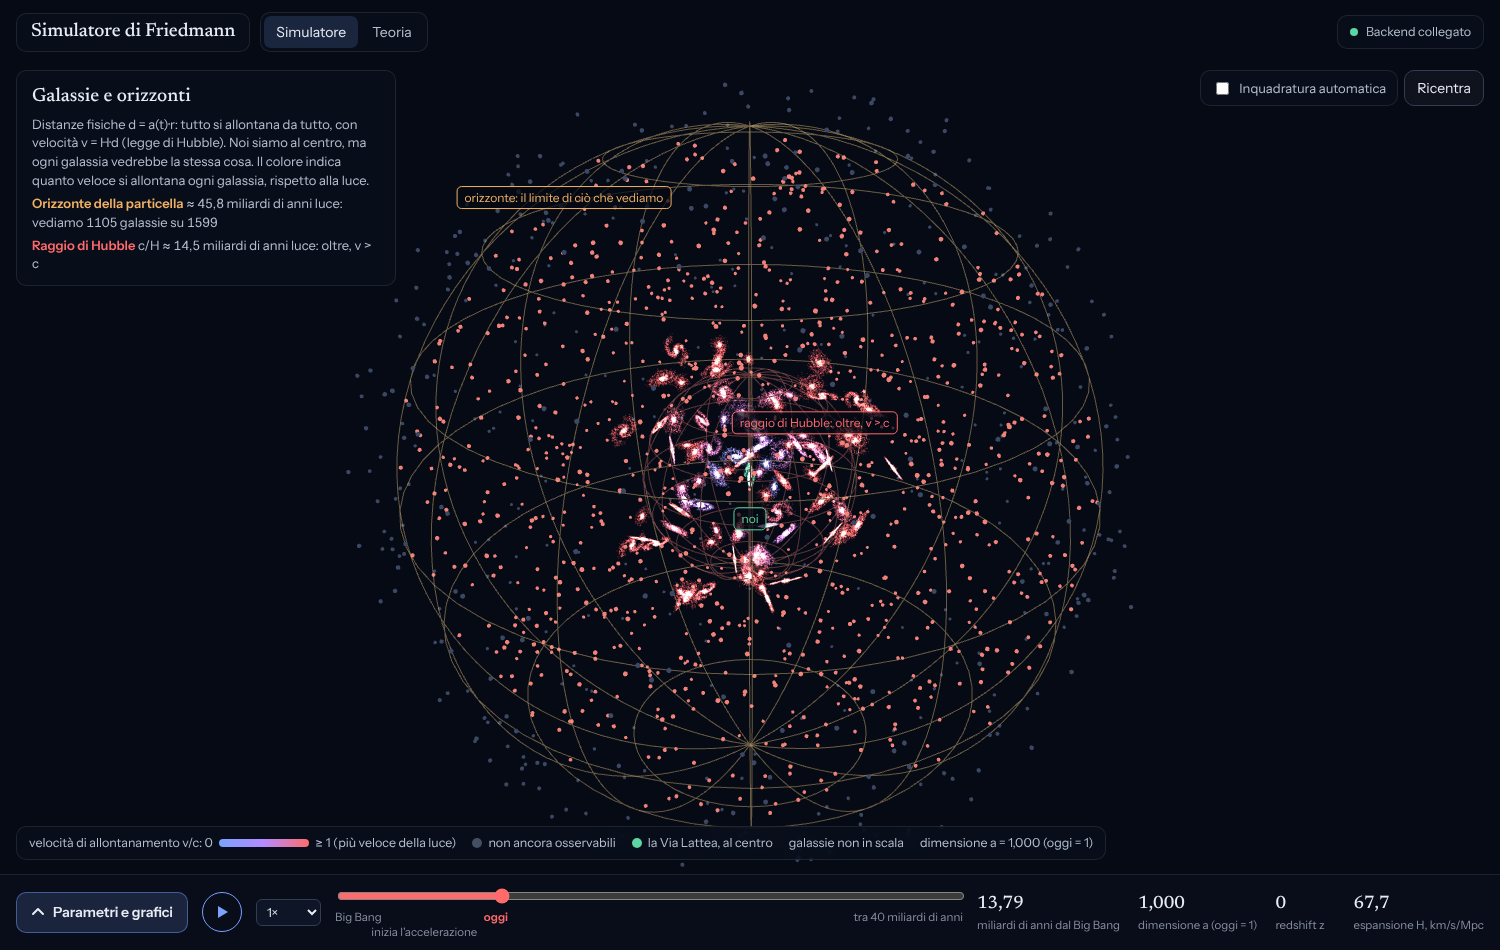
\includegraphics[width=\linewidth]{fig/galassie_oggi.png}
\caption{$\Lambda$CDM oggi. Noi siamo al centro; la sfera rossa è il raggio di Hubble, quella arancione l'orizzonte della particella. Il colore delle galassie è la velocità di allontanamento $v/c$.}
\end{figure}
Circa \num{1600} galassie occupano una regione di raggio $3{,}6\,c/H_0$; noi siamo al centro. Le distanze sono fisiche, $d=a(t)\,r$: facendo scorrere il tempo tutte le galassie si allontanano da tutte. Il colore indica la velocità di allontanamento rispetto alla luce, $v/c=H\,d/c$ (blu lento, rosso oltre $c$), e le galassie oltre l'orizzonte della particella sono grigie perché la loro luce non ci ha ancora raggiunto.
Per $\Lambda$CDM oggi si ottiene un orizzonte di circa 46 miliardi di anni luce e un raggio di Hubble di \num{14.5} miliardi di anni luce. Nell'era accelerata il raggio di Hubble resta quasi costante mentre le distanze crescono, e sempre più galassie si allontanano più velocemente della luce: è lo stesso meccanismo dell'inflazione.

Due scelte rappresentano la fisica:
\begin{itemize}
  \item la \textbf{posizione} delle galassie scala con $a(t)$, la loro \textbf{dimensione no}: le galassie sono sistemi legati dalla gravità e non partecipano all'espansione (le dimensioni sono ingrandite per essere visibili);
  \item prima di $a\approx1/11$ ($z\approx10$, qualche centinaio di milioni di anni dopo il Big Bang) le galassie non si sono ancora formate e la scena mostra solo materia diffusa.
\end{itemize}

\subsection{Riquadro delle equazioni}\label{sec:equazioni}
\begin{figure}[H]\centering
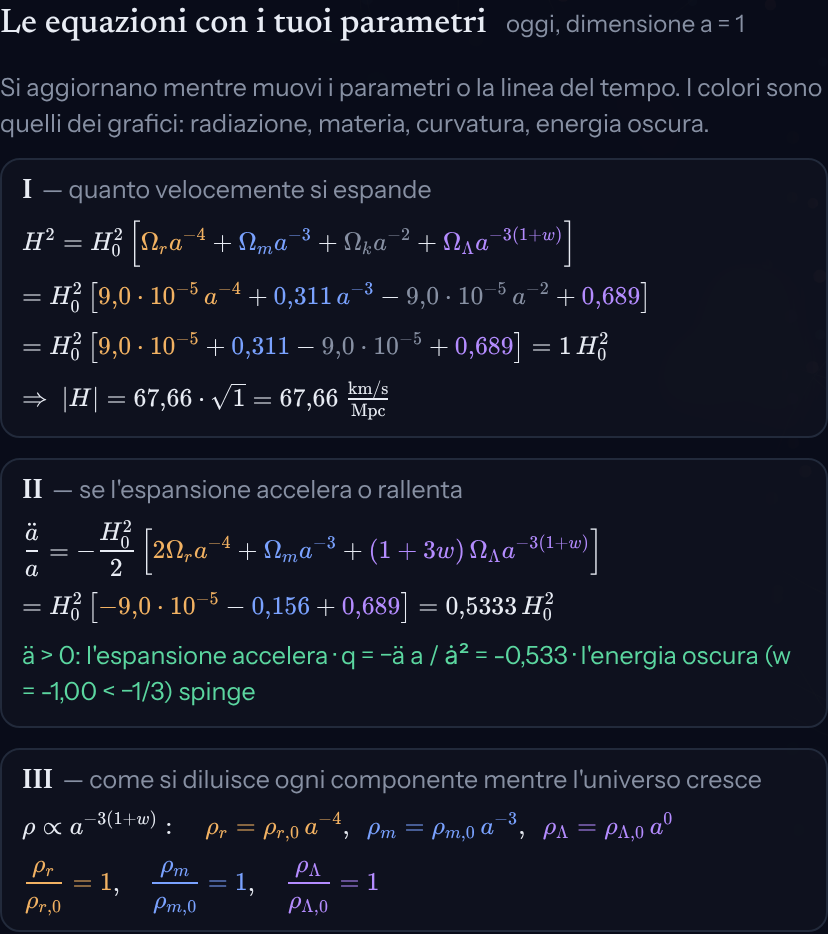
\includegraphics[width=0.62\linewidth]{fig/equazioni_live.png}
\caption{$\Lambda$CDM oggi: le tre equazioni con i parametri sostituiti. I colori sono quelli dei grafici (radiazione, materia, curvatura, energia oscura).}
\end{figure}
Il riquadro scrive le tre equazioni di Friedmann con i parametri del pannello e con il valore di $a$ al tempo del cursore, e si aggiorna in tempo reale:
\begin{itemize}
  \item \textbf{I}: ogni termine di $E^2(a)$ con il suo valore numerico, la somma e il valore di $H$;
  \item \textbf{II}: i contributi a $\ddot a/a$ (radiazione e materia frenano, l'energia oscura con $w<-1/3$ spinge), il segno dell'accelerazione e $q$;
  \item \textbf{III}: come si è diluita ogni componente, $\rho_i/\rho_{i,0}=a^{-3(1+w_i)}$.
\end{itemize}
Spostando un parametro o la linea del tempo si vede subito quale termine cambia e perché cambia il comportamento dell'universo.

\subsection{Grafici e linea del tempo}
\begin{figure}[H]\centering
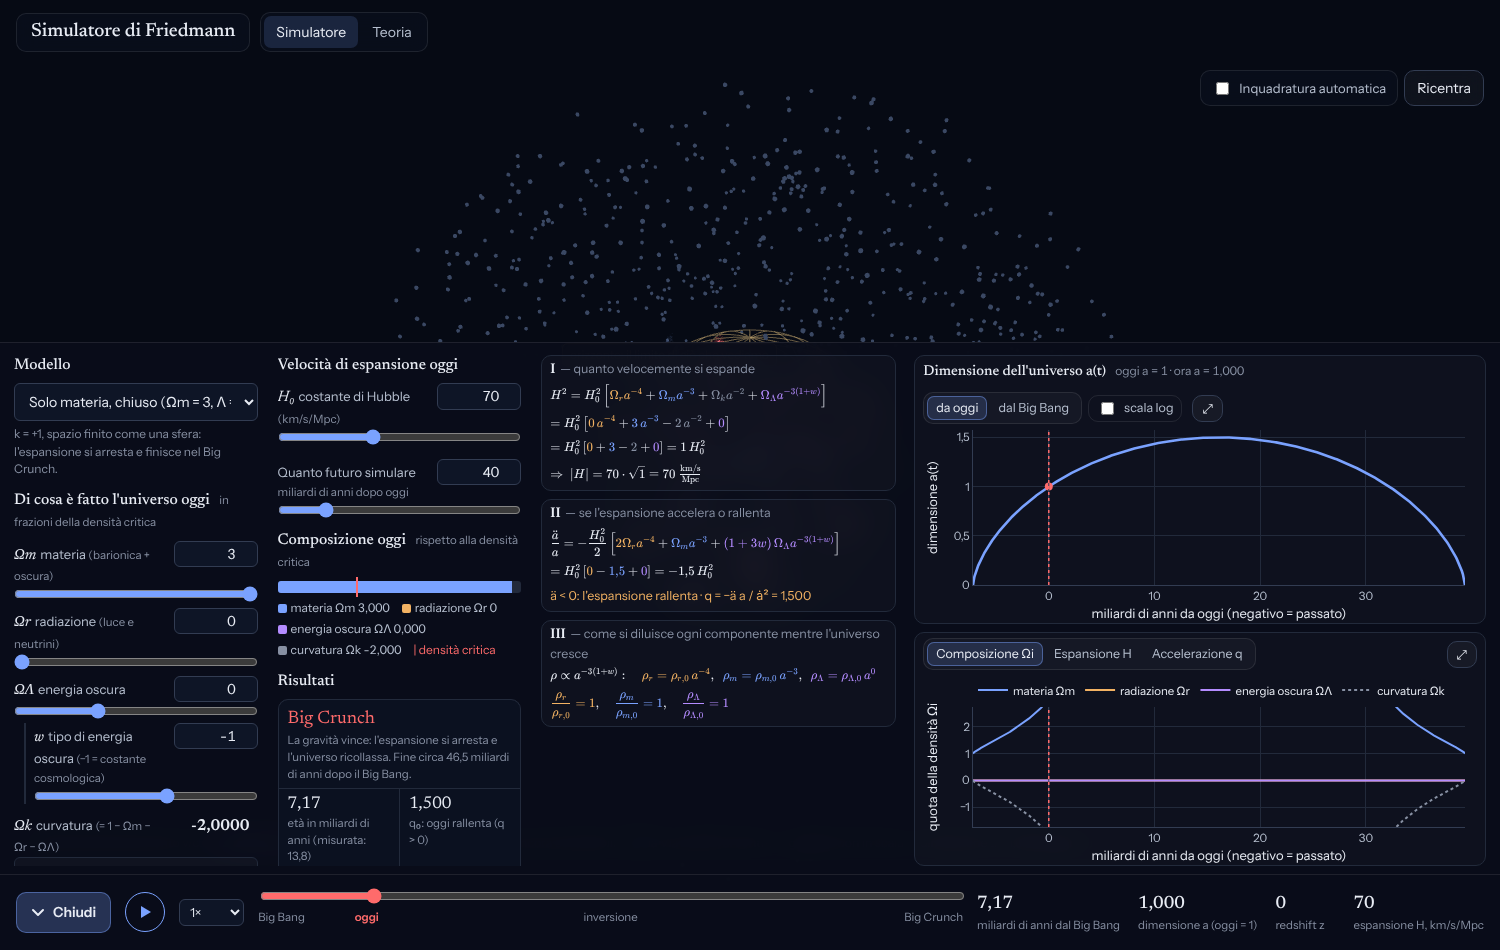
\includegraphics[width=\linewidth]{fig/pannello_chiuso.png}
\caption{Pannello aperto con il modello chiuso ($\Om=3$): parametri, $a(t)$ fino al Big Crunch e $\Omega_i(t)$.}
\end{figure}
Il grafico principale, ``Dimensione dell'universo'', mostra $a(t)$ (in funzione del tempo da oggi oppure dal Big Bang, anche in scala logaritmica), il secondo grafico mostra a scelta la composizione $\Omega_i(t)$, l'espansione $H(t)$ (con $|H|$ tratteggiato durante la contrazione) o l'accelerazione $q(t)$ (con l'area di accelerazione evidenziata). Nell'interfaccia i simboli sono sempre accompagnati da una parola che ne dice il significato, e i tempi sono scritti in miliardi di anni.
La linea del tempo, sempre visibile, ha un pulsante di riproduzione con velocità regolabile e segna gli eventi notevoli (Big Bang, inizio dell'accelerazione, oggi, inversione, Big Crunch); accanto mostra $t$, $a$, $z$ e $H$ al tempo corrente. Scena 3D, grafici e composizione seguono tutti lo stesso cursore.

\subsection{Pagina ``Teoria''}
Riassume le equazioni delle lezioni (sezione~2 di questa relazione) con pulsanti che caricano il modello corrispondente nel simulatore: per esempio ``Einstein--de Sitter'' accanto al problema dell'età, ``de Sitter: il raggio di Hubble si restringe'' accanto all'orizzonte.

% ===========================================================================
\section{Risultati e verifica}
% ===========================================================================

\begin{figure}[H]\centering
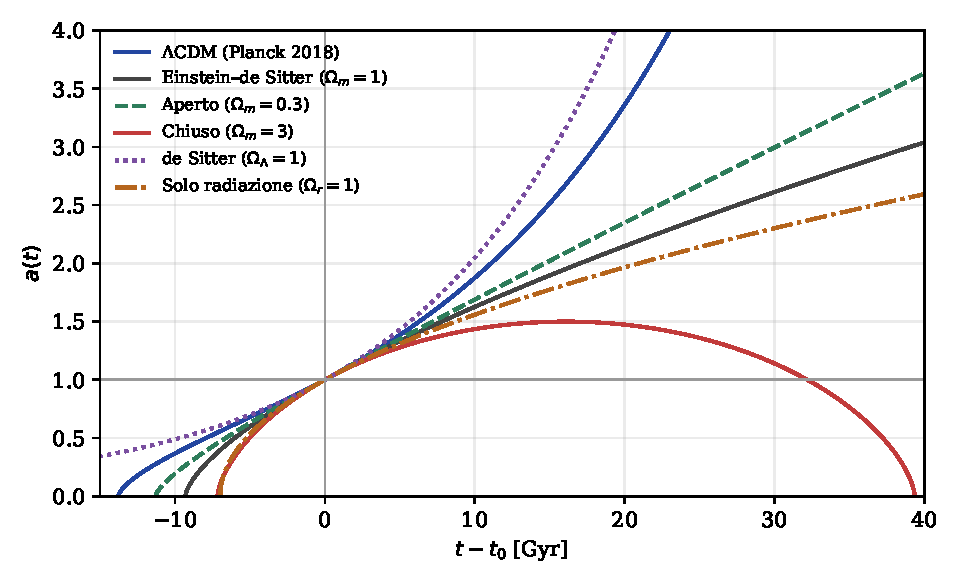
\includegraphics[width=0.82\linewidth]{fig/a_t_modelli.pdf}
\caption{Fattore di scala per i modelli delle lezioni, allineati a oggi ($a=1$ per $t=t_0$). Per $t<t_0$ si legge l'età (dove la curva tocca $a=0$): l'universo chiuso è il più giovane, de Sitter non ha un inizio.}
\end{figure}

\begin{figure}[H]\centering
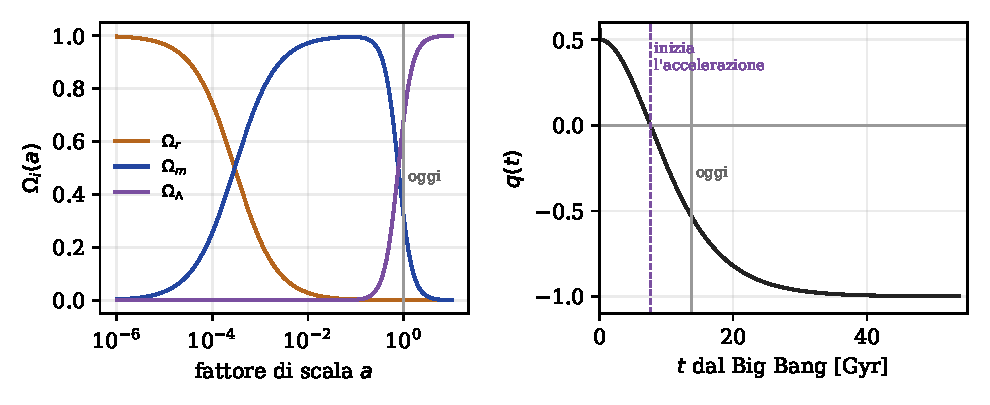
\includegraphics[width=0.95\linewidth]{fig/omega_q_lcdm.pdf}
\caption{$\Lambda$CDM. A sinistra: epoche di radiazione, materia ed energia oscura in funzione di $a$. A destra: il parametro di decelerazione cambia segno a $t\approx\SI{7.7}{Gyr}$ ($z\approx0{,}64$), cioè circa 6 miliardi di anni fa.}
\end{figure}

I risultati del server di calcolo sono stati confrontati con tre riferimenti indipendenti: le soluzioni analitiche, la libreria \texttt{astropy.cosmology} e l'integratore di riserva dell'interfaccia.

\begin{table}[H]\centering\small
\begin{tabular}{@{}lccccl@{}}
\toprule
Modello ($\Or=0$) & età attesa & età simulatore & $q_0$ & destino & note\\
\midrule
$\Lambda$CDM (Planck 2018) & 13,792 & 13,792 & $-0{,}533$ & accelerata & $z_{\text{acc}}=0{,}64$\\
Einstein--de Sitter & 9,312 & 9,312 & $0{,}500$ & eterna & $=2/(3H_0)$\\
Aperto, $\Om=0{,}3$ & 11,298 & 11,298 & $0{,}150$ & eterna & \\
Chiuso, $\Om=3$ & 7,170 & 7,170 & $1{,}500$ & Big Crunch & $a_{\max}=1{,}5$; $t_{\text{crunch}}=46{,}55$\\
Solo barioni & 13,331 & 13,331 & $0{,}015$ & eterna & \\
Fantasma, $w=-1{,}5$ & 14,273 & 14,273 & $-1{,}075$ & Big Rip & \\
Anti-de Sitter & 12,158 & 12,158 & $0{,}500$ & Big Crunch & $a_{\max}=\sqrt3$; $t_{\text{crunch}}=62{,}06$\\
Solo radiazione & 6,984 & 6,984 & $1{,}000$ & eterna & $=1/(2H_0)$\\
de Sitter & --- & --- & $-1{,}000$ & accelerata & passato infinito\\
Rimbalzo, $\OL=1{,}9$ & --- & --- & $-1{,}750$ & accelerata & $a_{\min}=0{,}611$\\
\bottomrule
\end{tabular}
\caption{Confronto con i valori di riferimento (tempi in \si{Gyr}, $H_0=70$ salvo $\Lambda$CDM). Le età attese sono calcolate con \texttt{astropy} e, dove esistono, con le formule analitiche; coincidono con il simulatore alla terza cifra decimale.}
\end{table}

\paragraph{Verifica esterna.} Lo stesso controllo si può fare con il calcolatore cosmologico di E.~L.~Wright (Wright 2006): con $H_0=67{,}66$, $\Om=0{,}3111$ e universo piatto l'età è di circa \SI{13.8}{Gyr}, come nel simulatore.

% ===========================================================================
\section{Limiti e possibili estensioni}
% ===========================================================================
\begin{itemize}
  \item Il modello è omogeneo e isotropo: descrive l'espansione media, non la formazione delle strutture. Le posizioni delle galassie nelle scene sono casuali e le loro dimensioni non sono in scala.
  \item La curvatura non è disegnata nella scena: si legge da $\Ok$, dal segno di $k$ e dal termine $\Ok a^{-2}$ della prima equazione.
  \item L'equazione di stato dell'energia oscura è costante; un'estensione naturale è $w(a)=w_0+w_a(1-a)$.
  \item Non sono calcolate le distanze osservative (di luminosità, di diametro angolare), che non sono state trattate nel corso; la struttura del codice permette di aggiungerle.
\end{itemize}

% ===========================================================================
\section{Conclusioni}
% ===========================================================================
Il simulatore risolve le equazioni di Friedmann per qualunque combinazione di materia, radiazione, energia oscura e curvatura, integrando la seconda equazione per seguire correttamente l'inversione dell'espansione e i casi senza Big Bang. Le visualizzazioni 3D mostrano i concetti delle lezioni --- l'espansione, la legge di Hubble, gli orizzonti, il ruolo di ogni termine delle equazioni --- legati in tempo reale alla soluzione numerica, e i risultati sono verificati con soluzioni analitiche e con strumenti di riferimento.

\appendix

% ===========================================================================
\section{Scaletta dell'orale}
% ===========================================================================
L'orale si apre con una breve introduzione teorica al fenomeno, poi mostra nel simulatore come cambia l'universo al variare dei parametri, collegando ogni risultato alla sua formula, e chiude con il funzionamento del programma. Il testo completo è nell'appendice~\ref{app:discorso}.

\begin{table}[H]\centering\small
\begin{tabularx}{\linewidth}{@{}l>{\raggedright\arraybackslash}Xl@{}}
\toprule
Parametro & Cosa succede nel simulatore & Formula\\
\midrule
$H_0$ più grande & universo più giovane & $t_0\propto 1/H_0$\\
$\Om<1,\ =1,\ >1$ & aperto / piatto / chiuso; con $\Om>1$ e $\OL=0$ Big Crunch & $\operatorname{sgn}(\Omega-1)=\operatorname{sgn}k$\\
$\OL=0$ ($\Om=1$) & età da 13,8 a \SI{9.3}{Gyr}, nessuna accelerazione & $t_0=2/(3H_0)$\\
$\OL$ grande & accelerazione; con troppa $\Lambda$ nessun Big Bang (rimbalzo) & $q_0=\Om/2-\OL$\\
$\OL<0$ & ricollasso anche con $k=-1$ (anti-de Sitter) & $a\propto\sin(\sqrt{0{,}5}\,H_0t)$\\
$w<-1/3$ & l'espansione accelera & $\ddot a>0\iff\rho+3p/c^2<0$\\
$w<-1$ & Big Rip in un tempo finito & $\rho\propto a^{-3(1+w)}$ cresce\\
solo $\Or$ & espansione più lenta & $a\propto t^{1/2}$\\
solo $\OL$ & espansione esponenziale, nessun inizio & $a\propto e^{Ht}$\\
\bottomrule
\end{tabularx}
\caption{Come cambia l'universo al variare dei parametri (traccia per le dimostrazioni dal vivo).}
\end{table}

\begin{table}[H]\centering\small
\begin{tabular}{@{}rlll@{}}
\toprule
& Parte & Durata & Nel simulatore\\
\midrule
0--2 & Il fenomeno e le equazioni & 3 min & ---\\
3--4 & $\Lambda$CDM e la curvatura & 1,5 min & galassie, riquadro equazioni\\
5--7 & Età, Big Crunch, accelerazione & 3 min & pannello, grafici $a(t)$, $H$, $q$\\
8 & Galassie e orizzonti & 1,5 min & Galassie e orizzonti\\
9--10 & Funzionamento, verifica, chiusura & 1,5 min & riquadro delle equazioni\\
\bottomrule
\end{tabular}
\caption{Tempi indicativi (circa 10 minuti). In due si può alternare: uno spiega la formula, l'altro la mostra nel simulatore.}
\end{table}

% ===========================================================================
\section{Discorso completo}\label{app:discorso}
% ===========================================================================
Le righe precedute da {\color{blu}$\blacktriangleright$} sono le azioni da fare sul simulatore.
% ---------------------------------------------------------------------------
%  Testo del discorso per l'orale: incluso sia in relazione.tex (appendice)
%  sia in discorso.tex (versione da stampare e imparare).
%  Le righe con il triangolo blu (\demo) sono azioni da fare sul simulatore, non da dire.
% ---------------------------------------------------------------------------

\subsection*{0. Apertura \hfill\normalfont\small 30 s}
Buongiorno. Il nostro progetto è un simulatore della dinamica dell'universo: dati i contenuti dell'universo di oggi, risolve le equazioni di Friedmann e ne mostra il passato e il futuro, anche in tre dimensioni.
Prima introduciamo brevemente la fisica, poi mostriamo nel simulatore come ogni risultato discende dalle formule, e infine spieghiamo come funziona il programma.

\demo{Avviare con \texttt{avvia.bat} prima di entrare: si apre su $\Lambda$CDM, vista ``Spazio curvo''.}

\subsection*{1. Il fenomeno: l'universo si espande \hfill\normalfont\small 1 min}
Osservando le galassie lontane si vede che si allontanano da noi con una velocità proporzionale alla distanza: è la legge di Hubble, $v = H_0\, d$.
Questo non significa che noi siamo al centro: ogni galassia vede tutte le altre allontanarsi. Non sono le galassie a muoversi nello spazio, è lo spazio stesso che si dilata.

Per descriverlo si usa un solo numero che dipende dal tempo, il \textbf{fattore di scala} $a(t)$. Ogni galassia ha una coordinata comovente $r$ fissa, e la sua distanza fisica è $d = a(t)\,r$. Per convenzione $a = 1$ oggi; $a = 1/2$ vuol dire che le distanze erano la metà.
Derivando, $v = \dot a\, r = \frac{\dot a}{a}\, d$: la legge di Hubble viene fuori da sola, con $H = \dot a / a$.

Anche il redshift si legge con $a$: la luce si allunga insieme allo spazio, quindi $1 + z = 1/a(t_e)$. Una galassia a $z = 1$ ha emesso la luce quando l'universo era grande la metà.

\subsection*{2. Le equazioni di Friedmann \hfill\normalfont\small 1 min 30 s}
Se l'universo su grande scala è omogeneo e isotropo --- il principio cosmologico --- la geometria è quella di Robertson--Walker e dipende solo da $a(t)$ e dal segno della curvatura $k$: $k=0$ spazio piatto, $k=+1$ chiuso come una sfera, $k=-1$ aperto come una sella.

Inserendo questa metrica nelle equazioni di Einstein si ottengono le equazioni di Friedmann. La prima,
\[
  H^2 = \frac{8\pi G}{3}\rho - \frac{kc^2}{a^2},
\]
lega la velocità di espansione a quello che c'è nell'universo e alla curvatura. La seconda,
\[
  \frac{\ddot a}{a} = -\frac{4\pi G}{3}\left(\rho + \frac{3p}{c^2}\right),
\]
dice se l'espansione rallenta o accelera. La terza è la conservazione dell'energia e, con l'equazione di stato $p = w\rho c^2$, dà $\rho \propto a^{-3(1+w)}$.

Quindi ogni ingrediente si diluisce in modo diverso: la radiazione come $a^{-4}$, la materia come $a^{-3}$, la costante cosmologica resta costante. Per questo nella storia dell'universo domina prima la radiazione, poi la materia, oggi l'energia oscura.

Definendo la densità critica $\rho_c = 3H^2/8\pi G$ e $\Omega = \rho/\rho_c$, la prima equazione diventa $\Omega - 1 = kc^2/(a^2H^2)$: il segno di $\Omega - 1$ è il segno della curvatura. Con più densità di quella critica l'universo è chiuso, con meno è aperto.
In conclusione, i parametri di oggi --- $H_0$, $\Omega_m$, $\Omega_r$, $\Omega_\Lambda$ e $w$ --- determinano tutta la storia dell'universo. Il simulatore fa esattamente questo.

\subsection*{3. Il nostro universo, \texorpdfstring{$\Lambda$}{Lambda}CDM \hfill\normalfont\small 1 min}
\demo{Vista ``Spazio curvo'', modello $\Lambda$CDM. Premere play.}
Questo è il modello standard, con i parametri di Planck: circa 31\% di materia e 69\% di energia oscura, quindi $\Omega \approx 1$ e lo spazio è piatto.
La griglia rappresenta lo spazio con una dimensione in meno, perché uno spazio curvo tridimensionale non si può disegnare. Le galassie sono ferme sulla griglia, cioè hanno coordinate comoventi fisse: è la griglia che si dilata come $a(t)$.
Le galassie si allontanano ma non diventano più grandi, perché sono tenute insieme dalla gravità. E prima di $z \approx 10$ non ci sono: non si erano ancora formate.

\demo{Aprire ``Parametri e grafici'': indicare l'età.}
L'età che risulta è 13,8 miliardi di anni, come quella misurata.

\subsection*{4. Le tre geometrie \hfill\normalfont\small 30 s}
\demo{Pulsante ``Confronta $k = +1, 0, -1$''.}
Qui ci sono le tre geometrie allo stesso fattore di scala: la sfera per $\Omega > 1$, il piano per $\Omega = 1$, la sella per $\Omega < 1$. È la relazione $\operatorname{sgn}(\Omega - 1) = \operatorname{sgn}(k)$, e il segno non cambia nel tempo.

\subsection*{5. Il problema dell'età \hfill\normalfont\small 1 min}
\demo{``Aggiungi al confronto'' su $\Lambda$CDM, poi modello Einstein--de Sitter.}
Ora togliamo l'energia oscura: solo materia, universo piatto. È il modello di Einstein--de Sitter. La prima equazione si risolve a mano: $a(t) \propto t^{2/3}$ e quindi $H = 2/(3t)$, cioè l'età è $t_0 = 2/(3H_0)$.
Il simulatore infatti dà 9,3 miliardi di anni. Ma ci sono stelle più vecchie di 10 miliardi di anni: è il problema dell'età. Senza energia oscura i conti non tornano.
Nel grafico si vede anche perché: la curva di $a(t)$ è concava, l'espansione ha sempre rallentato, quindi andando indietro arriva prima a zero. Quel punto, dove $a = 0$ e la densità è infinita, è il Big Bang.

\subsection*{6. Il Big Crunch \hfill\normalfont\small 1 min}
\demo{Modello ``Chiuso, solo materia'' ($\Omega_m = 3$). Mostrare $a(t)$ e $H(t)$.}
Se la densità supera quella critica, senza energia oscura, l'universo è chiuso. L'espansione rallenta fino a fermarsi, a $a_{\max} = \Omega_m/(\Omega_m - 1) = 1{,}5$, poi l'universo ricollassa: il Big Crunch, qui dopo circa 47 miliardi di anni dal Big Bang. Nel grafico $H$ diventa negativo.
Questo spiega una scelta del programma: la prima equazione dà $\dot a$ come una radice quadrata, sempre positiva, quindi non può descrivere un universo che si ferma e torna indietro. Per questo integriamo la seconda equazione, che contiene $\ddot a$ e segue l'inversione; la prima serve solo per le condizioni iniziali.

\subsection*{7. L'espansione accelerata \hfill\normalfont\small 1 min}
\demo{Tornare a $\Lambda$CDM, grafico ``$q(t)$''.}
Il parametro di decelerazione $q = -\ddot a\, a/\dot a^2$ è positivo quando l'espansione rallenta. Dalla seconda equazione, l'espansione accelera solo se $\rho + 3p/c^2 < 0$, cioè con $w < -1/3$: la materia non può farlo, l'energia oscura con $w = -1$ sì.
Nel nostro universo $q$ cambia segno circa 6 miliardi di anni fa, a $z \approx 0{,}6$: da lì l'energia oscura domina. È quello che hanno misurato con le supernovae nel 1998. Oggi $q_0 \approx -0{,}53$.

\demo{Modello de Sitter.}
Se c'è solo costante cosmologica, $H$ è costante e $a \propto e^{Ht}$: andando indietro $a$ non arriva mai a zero, quindi non c'è Big Bang e l'età non è definita. È così che va l'inflazione nell'universo primordiale, ed è il futuro del nostro universo.

\demo{Facoltativo: $w = -1{,}5$ dal cursore.}
Se $w < -1$ la densità dell'energia oscura aumenta con l'espansione e l'universo si strappa in un tempo finito: il Big Rip.

\subsection*{8. Galassie e orizzonti \hfill\normalfont\small 1 min 30 s}
\demo{Vista ``Galassie e orizzonti'', $\Lambda$CDM oggi; poi ``Comoventi'' e play nel futuro.}
Qui siamo al centro, e il colore delle galassie indica la velocità di recessione $v = H\, d$.
La sfera rossa è il raggio di Hubble, $c/H$, circa 14,5 miliardi di anni luce: oltre, le galassie si allontanano più veloci della luce. Non viola la relatività, perché è lo spazio che si espande.
La sfera arancione è l'orizzonte della particella, $\chi_p = c\int dt/a$: la distanza da cui la luce ha fatto in tempo ad arrivarci dal Big Bang. Oggi è circa 46 miliardi di anni luce: molto più di 13,8 miliardi di anni luce, perché mentre la luce viaggiava lo spazio si è dilatato. Le galassie grigie sono oltre l'orizzonte e non le vediamo ancora.
In coordinate comoventi, andando nel futuro, il raggio di Hubble si restringe: sempre più galassie escono dalla nostra portata. È lo stesso meccanismo dell'inflazione, che risolve il problema dell'orizzonte.

\subsection*{9. Come funziona il simulatore e verifica \hfill\normalfont\small 1 min}
\demo{Vista ``Superficie $a(t)$'', famiglia ``da aperto a chiuso''.}
Questa superficie riassume tutto: ogni sezione è una soluzione delle equazioni di Friedmann al variare di $\Omega_m$. Per $\Omega_m > 1$ le curve tornano a zero: il Big Crunch.

Il programma ha due parti. Il server di calcolo, in Python, integra la seconda equazione partendo da oggi, con $a = 1$ e $\dot a = H_0$, sia all'indietro fino al Big Bang sia in avanti, con un integratore Runge--Kutta adattivo di SciPy; riconosce gli eventi notevoli e classifica l'origine e il destino. L'interfaccia, nel browser, mostra i risultati in 3D e nei grafici.
Abbiamo verificato i risultati con le soluzioni analitiche --- Einstein--de Sitter, solo radiazione, universo chiuso, anti-de Sitter --- e con la libreria \texttt{astropy}: le età coincidono alla terza cifra decimale.

\subsection*{10. Chiusura \hfill\normalfont\small 20 s}
In sintesi: con le sole equazioni di Friedmann e cinque parametri si ottengono il Big Bang, il ricollasso, l'espansione eterna e quella accelerata, e il simulatore mostra ogni caso collegato alla sua formula.
I limiti sono che il modello descrive l'espansione media e non la formazione delle strutture, e che la curvatura è rappresentata con una superficie in due dimensioni.
Grazie, siamo pronti per le domande.


% ===========================================================================
\section{Domande probabili}
% ===========================================================================

\begin{orale}
\textbf{Perché non integra direttamente la prima equazione?}\\
Perché dà $\dot a=H_0a\sqrt{E^2(a)}$, sempre positivo: non può descrivere un universo che smette di espandersi e ricollassa. La seconda equazione contiene $\ddot a$ e segue l'inversione; la prima serve per le condizioni iniziali ($\dot a(t_0)=H_0$).
\end{orale}

\begin{orale}
\textbf{Anche le galassie (e il Sistema Solare) si espandono?}\\
No: sono sistemi legati dalla gravità e la loro dinamica interna domina sull'espansione. Si allontanano le une dalle altre, ma non crescono di dimensione: nel simulatore cambia la posizione, non la grandezza.
\end{orale}

\begin{orale}
\textbf{Cosa indica il colore delle galassie?}\\
La velocità con cui si allontanano, divisa per quella della luce: $v/c=H\,d/c$. Le galassie rosse sono oltre il raggio di Hubble e si allontanano più veloci della luce, cosa permessa perché è lo spazio che si espande; quelle grigie sono oltre l'orizzonte e la loro luce non ci ha ancora raggiunto.
\end{orale}

\begin{orale}
\textbf{Cosa succede se $\Omega>1$?}\\
Per la (\ref{eq:segno}) $k=+1$: lo spazio è chiuso e, senza $\Lambda$, l'espansione si arresta a $a_{\max}=\Om/(\Om-1)$ e l'universo ricollassa. Con abbastanza $\Lambda$ anche un universo chiuso può espandersi per sempre.
\end{orale}

\begin{orale}
\textbf{Che differenza c'è tra raggio di Hubble e orizzonte della particella?}\\
Il raggio di Hubble $c/H$ è dove la velocità di recessione vale $c$; l'orizzonte della particella è la distanza da cui la luce ha fatto in tempo ad arrivarci dal Big Bang. Oggi l'orizzonte (circa 46 miliardi di anni luce) è più grande del raggio di Hubble (circa 14,5): vediamo galassie che oggi si allontanano più veloci della luce, perché la luce che riceviamo è partita quando erano più vicine.
\end{orale}

\begin{orale}
\textbf{Si può simulare l'universo statico di Einstein?}\\
No, con questi parametri: il simulatore fissa le condizioni a oggi con $H_0>0$, mentre un universo statico ha $H=0$. Si può però mostrare che l'equilibrio richiede $\Lambda c^2=4\pi G\rho$ e $k=+1$, ed è instabile.
\end{orale}

\begin{orale}
\textbf{Come sa che i risultati sono giusti?}\\
Per i casi con soluzione analitica (Einstein--de Sitter, radiazione, chiuso, anti-de Sitter) il confronto è esatto; per gli altri l'età coincide con \texttt{astropy} alla terza cifra decimale, e il risultato di $\Lambda$CDM (\SI{13.79}{Gyr}) coincide con il valore di Planck 2018.
\end{orale}

% ===========================================================================
\begin{thebibliography}{99}\small
\bibitem{lezioni} C.~Daffara, \emph{Elementi di Cosmologia e Relatività Generale}, lezioni 1--3, Università di Verona, A.A.\ 2025/2026.
\bibitem{ryden} B.~Ryden, \emph{Introduction to Cosmology}, 2\textsuperscript{a} ed., Cambridge University Press, 2017.
\bibitem{friedmann} A.~Friedmann, Über die Krümmung des Raumes, \emph{Zeitschrift für Physik} \textbf{10}, 377--386 (1922).
\bibitem{cpt} S.~M.~Carroll, W.~H.~Press, E.~L.~Turner, The cosmological constant, \emph{Annual Review of Astronomy and Astrophysics} \textbf{30}, 499--542 (1992).
\bibitem{riess} A.~G.~Riess et al., Observational evidence from supernovae for an accelerating universe and a cosmological constant, \emph{The Astronomical Journal} \textbf{116}, 1009 (1998).
\bibitem{perlmutter} S.~Perlmutter et al., Measurements of $\Omega$ and $\Lambda$ from 42 high-redshift supernovae, \emph{The Astrophysical Journal} \textbf{517}, 565 (1999).
\bibitem{caldwell} R.~R.~Caldwell, M.~Kamionkowski, N.~N.~Weinberg, Phantom energy: dark energy with $w<-1$ causes a cosmic doomsday, \emph{Physical Review Letters} \textbf{91}, 071301 (2003).
\bibitem{planck} Planck Collaboration, Planck 2018 results. VI. Cosmological parameters, \emph{Astronomy \& Astrophysics} \textbf{641}, A6 (2020).
\bibitem{wright} E.~L.~Wright, A cosmology calculator for the World Wide Web, \emph{Publications of the Astronomical Society of the Pacific} \textbf{118}, 1711 (2006).
\bibitem{scipy} P.~Virtanen et al., SciPy 1.0: fundamental algorithms for scientific computing in Python, \emph{Nature Methods} \textbf{17}, 261--272 (2020).
\bibitem{astropy} Astropy Collaboration, The Astropy Project: sustaining and growing a community-oriented open-source project, \emph{The Astrophysical Journal} \textbf{935}, 167 (2022).
\bibitem{three} Three.js, libreria JavaScript per la grafica 3D, \url{https://threejs.org}.
\end{thebibliography}

\end{document}
